\section{Analysis on request textual content}
In this section, we perform analysis on the two text-based attributes in our dataset, i.e. \textit{request\_title} and \textit{request\_text\_edit\_aware}. These attributes contain the title and textual body of each request. Most of decision will be based upon the contents of these two attributes.

\subsection{Textual content preprocessing}

In order to perform analysis, we need to do preprocessing steps on these two attributes. First, we observed that the title of a request somewhat summaries the content in the request text, thus, analyze these two text attributes separately it is a good idea to combine title and the request text in to a single text document. Next, we tokenized a document into words using simple regular expression to find words: \verb|[a-z][a-z'\-_]+[a-z])||\verb|([a-z]+)|. In language, there are several stop words which are words that have meaning too general e.g.\texttt{you, me}, etc. These words ofter do not have predictive power because they occur in both successful and unsuccessful requests. Thus, after tokenizing words, we removed stop words from documents. After stop words removal step, there are 12930 distinct words occur in the corpus, 6358 distinct words only occur in successful requests, and 10823 distinct words only occur in unsuccessful requests.     

\subsection{Empirical analysis on words}

When looking at request text, we are often interested in keywords or topics that are associated with successful requests and unsuccessful requests. These keywords can give some insights about which kind of requests often receive pizza and which kind of requests do not. We defined ``positive'' keywords as the words that often occur in successful request but rarely occur in the unsuccessful requests, and ``negative'' keywords as the words that often occur in unsuccessful request but rarely occur in the successful requests. To find top ``positive'' words, we ranked all words based on \textit{constract score}:

\begin{equation}
	\phi = \frac{p}{n}(p-n)
\end{equation}    

where $p$ and $n$ are correspondingly the counts of successful and unsuccessful requests containing the word. After compute \textit{constract score}, we can select top-$k$ words based on the ranking of scores. The process of finding top ``negative'' words as similar but in the \textit{constract score} formula we exchange $n$ and $p$. Figure \ref{top} shows top-30 ``positive'' words and ``negative'' words. From the figures, there are several interesting points we can see. Top ``positive'' words contains several words related to children topic like \texttt{\{disney, daughter's, babies\}}, location topic like \texttt{\{toledo, wellington, asian\}}. This suggests that requests mentioned about those topics tend to be successful. Top ``negative'' words contains several words related to money topic like \texttt{\{money, penny, penniless\}}, relationship topic like \texttt{\{love, friend, girlfriends, coworkers\}}, bad activities like \texttt{\{frunk, smoking, broke, dumped\}}, and locations like \texttt{\{island, alaska\}}. This suggests that requests mentioned about those topics tend to be unsuccessful.

\begin{figure}
	\centering
	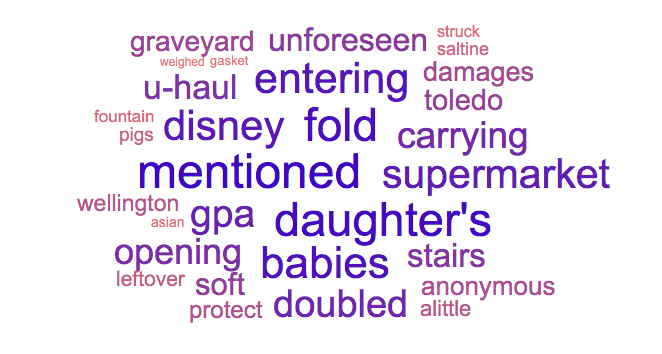
\includegraphics[width=0.40\textwidth]{data/positive}
	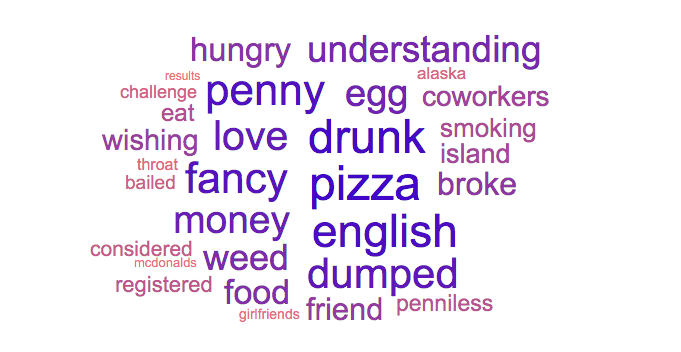
\includegraphics[width=0.40\textwidth]{data/negative}
	\caption{Top ``positive'' words and top ``negative'' words}
	\label{top}
\end{figure}

\subsection{Outcome prediction}
In second analysis, we perform a classification task using text attributes. For the prediction model, we built the same logistic regression model (maximum entropy classifier) as the model for requester information attributes. We also used the same cross validation settings and folds as the previous classification experiment. Table \ref{confusion2} shows a confusion matrix for the same fold as the previous experiment but now using text attributes. In the result, the overall $F$-measure are \textbf{0.31}. The result now is much better than using requester information attributes. The classifier now can classify both successful and unsuccessful request.

 \begin{table}[]
	\centering
	\caption{The confusion matrix for a fold in the cross validation (using text attributes)}
	\label{confusion2}
	\begin{tabular}{|c|c|c|c|}
		\hline
		\multicolumn{2}{|c|}{\multirow{2}{*}{}}                & \multicolumn{2}{c|}{Actual}                            \\ \cline{3-4} 
		\multicolumn{2}{|c|}{}                                 & \multicolumn{1}{c|}{TRUE} & \multicolumn{1}{c|}{FALSE} \\ \hline
		\multicolumn{1}{|c|}{\multirow{2}{*}{Predict}} & TRUE  & 27                         & 79                          \\ \cline{2-4} 
		\multicolumn{1}{|c|}{}                         & FALSE & 33                        & 265                        \\ \hline
	\end{tabular}
\end{table} 
